%% ==============================
\chapter{\iflanguage{ngerman}{Design}{Concept}}
\label{sec:concept}
%% ==============================


Nachdem im vorherigen Kapitel die verschieden Methoden die genutzt werden vorgestellt wurden, beschäftigt sich dieser Abschnitt mit dem Softwaredesign.
\newline
Die Implementierung dieser Bachelorarbeit teilt sich dabei in zwei verschieden Programme auf. Zum einen den sogenannten \textit{VolumeRenderHelper}, der für das Laden, Umwandeln, Verarbeiten und Speichern der Volumendaten zuständig ist.
Zum anderen das Unityprogramm \textit{VolumeRenderer}, welches zur Visualisierung der vom \textit{VolumeRenderHelper} erzeugten Daten dient. Diese beiden Programme existierten bereits vor dieser Arbeit und sind in Vorarbeiten des IPRs entstanden.


In dieser Bachelorarbeit wurde der \textit{VolumeRenderHelper} um die vorgestellte Transferfunktion erweitert und der \textit{VolumeRenderer} geringfügig angepasst. Da beide Programme in \textit{C\#} geschrieben sind, wurden auch der Code, der im Laufe dieser Bachelorarbeit entstand, in \textit{C\#} geschrieben. Als Entwicklerumgebung wurde \textit{Visual Studio 2017} von Microsoft verwendet. Die Beiden Programme werden im folgenden als Helper und Renderer bezeichnet. Weiterhin wurde ein Pythonskript \textit{PlotHelper} geschrieben, um LH-Histogramme anzuzeigen.


Anfangs liegen die CT-Daten der Volumen in mehreren Dateien als Schnittbilder im DICOM Format vor. Diese werden mithilfe der \textit{Medical Imaging Interaction Toolkit} (kurz: \textit{MITK}) \textit{Workbench} \cite{mitk} zu einer einzelnen Datei im .nrrd Format umgewandelt, da Volumen nur in diesem Format, oder als binäre Datei, vom Helper eingelesen werden können.
\textit{MITK} ist ein kostenloses open-source System zur Entwicklung von medizinischer Bildverarbeitungssoftware und wurde vom Deutschen Krebsforschungszentrum entwickelt. Dessen \textit{Workbench} bietet zum einen, das eben vorgestellte Laden und Umwandeln von DICOM Dateien, zum anderen auch diverse Segmentierungstools.


Die Darstellung von Volumendaten ist über den Renderer in Unity möglich. Der Benutzer hat hierbei mehrere Möglichkeiten Eingaben über Parameterfelder, wie beispielsweise in \autoref{fig:unity_para} zu sehen, oder mithilfe der Tastatur zu machen und mit der Visualisierung zu interagieren. Zunächst muss er jedoch in das Parameterfeld \textit{Binary Data} via drag and drop eine binäre Volumendatei ziehen.
Anschließend kann die Visualisierung gestartet werden. Hierbei hat der Nutzer die Möglichkeit die Kamera mit den Tasten $W$ $A$ $S$ $D$ zu bewegen als auch mit den seitlichen Pfeiltasten sowie der $Q$ und $E$ Taste das Volumen um verschiedene Achsen zu drehen. Die Position der Kamera sowie die Drehung des Volumens, kann ebenfalls durch entsprechende Parameterfelder verändert werden.
Die Volumen, werden als Graubilder dargestellt, wobei die Helligkeit der einzelnen Voxel abhängig vom Intensitätswert bestimmt wird. Dabei kann der User über ein weiteres Parameterfeld entscheiden ob der Größte, der Kleinste, der Erste oder die Summe aller gefunden Voxel als Wert für die Farbgebung benutzt wird. Der Standard ist hierbei, dass des maximale Wert genommen wird .
\newline
Des Weiteren kann der Nutzer einen Threshold setzen, bei dem alle Voxel die einen Intensitätswert niedriger als diesen haben für die Visualisierung ignoriert werden.
Es existieren noch deutlich mehr Eingabefelder, mit denen der Benutzer die Darstellung des Volumens verändern und anpassen kann. Diese werden jedoch, da sie im Kontext dieser Bachelorarbeit von wenig Interesse sind, nicht alle vorgestellt.


\begin{figure}
\centering
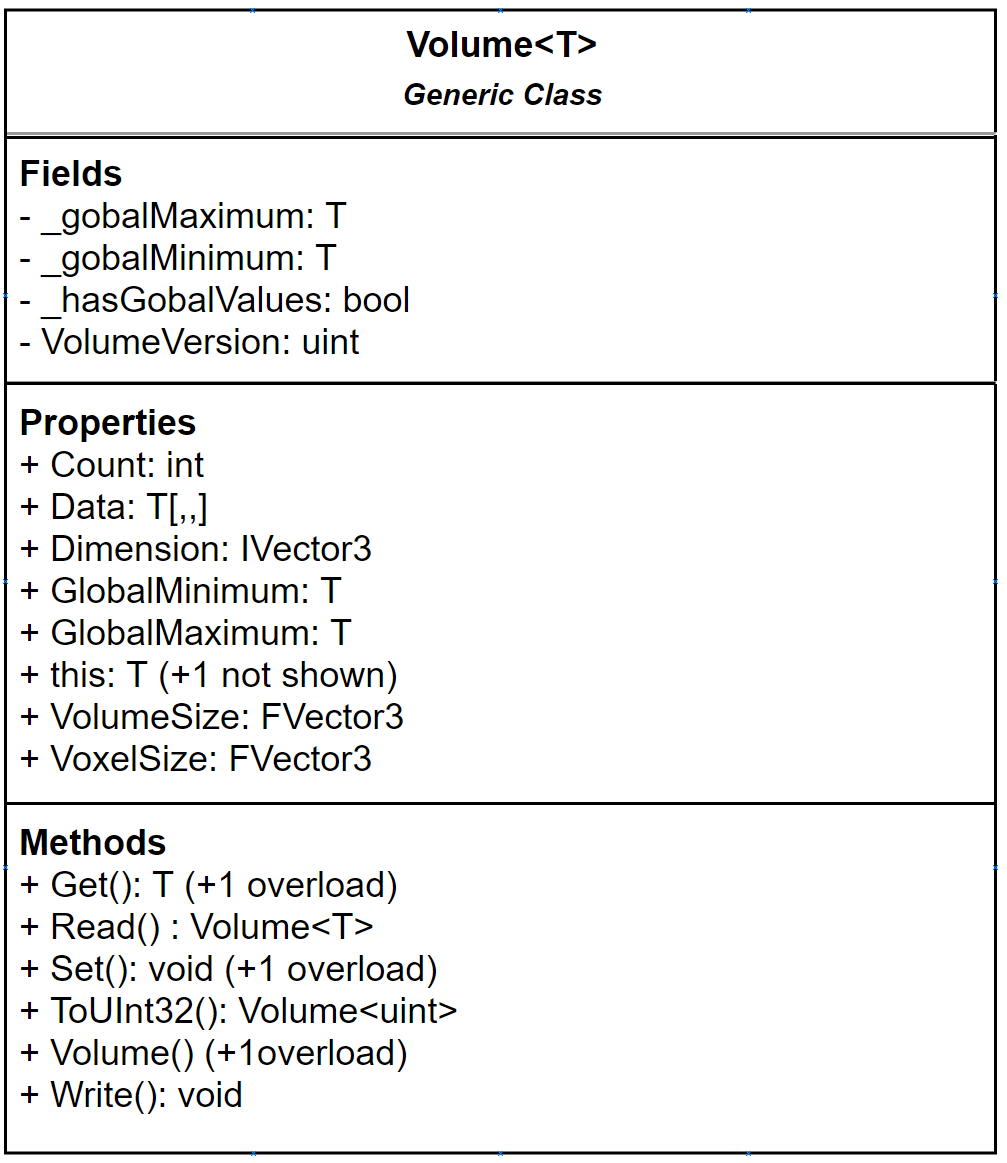
\includegraphics[width=0.6\textwidth]{Logos/Volume_UML.PNG}
\caption{UML-Diagramm des Volumens} 
\label{fig:volume_uml} 
\end{figure}


Die in der Vorarbeit bereits vorhandene interne Speicherung des Volumens im Helper wird mit der generischen Klasse \textit{Volume} umgesetzt, deren Felder, Attribute und Methoden in \autoref{fig:volume_uml} zu sehen sind. Diese besitzt ein dreidimensionalen Array vom angegebenen generischen Datentyp, sowie Informationen über das Volumen, wie zum Beispiel Größe der Voxel oder Anzahl der Elemente pro Achse.
Des Weiteren bietet die Klasse verschieden Funktionen um Informationen auszulesen oder zu bearbeiten. Zur Darstellung von dreidimensionale Koordinaten, werden die Klassen \textit{IVector3} und \textit{FVector3} benutzt. Diese stellen Vektoren dar, die entweder Integer, Ganzzahlen, oder Float, Dezimalzahlen, als $x$, $y$ und $z$ Werte speichern.


Die Interaktion des Benutzers mit dem Helper findet über eine Kommandozeile statt. Hierbei hat der Anwender die Befehle \textit{Load}, \textit{Dump}, \textit{Resample}, \textit{Info}, \textit{Write}, \textit{LHHistogram}, \textit{ClusterVolume} und \textit{MergeCluster} zur Auswahl. Jedes Modul hat dabei spezifische Parameter, die beim Aufruf angegeben werden müssen. Wird ein Befehl mit einem Help dahinter aufgerufen, wird die richtige Benutzung des Moduls erklärt.
Die vorgestellten Module erben dabei alle von der abstrakten \textit{BaseModule} Klasse, die es ihnen vorschreibt, eine \textit{Call} sowie eine \textit{PrintHelp} Methode zu implementieren. Dies ist im UML-Diagramm in \autoref{fig:modul_uml} zu sehen.


\begin{figure}[h]
\centering 
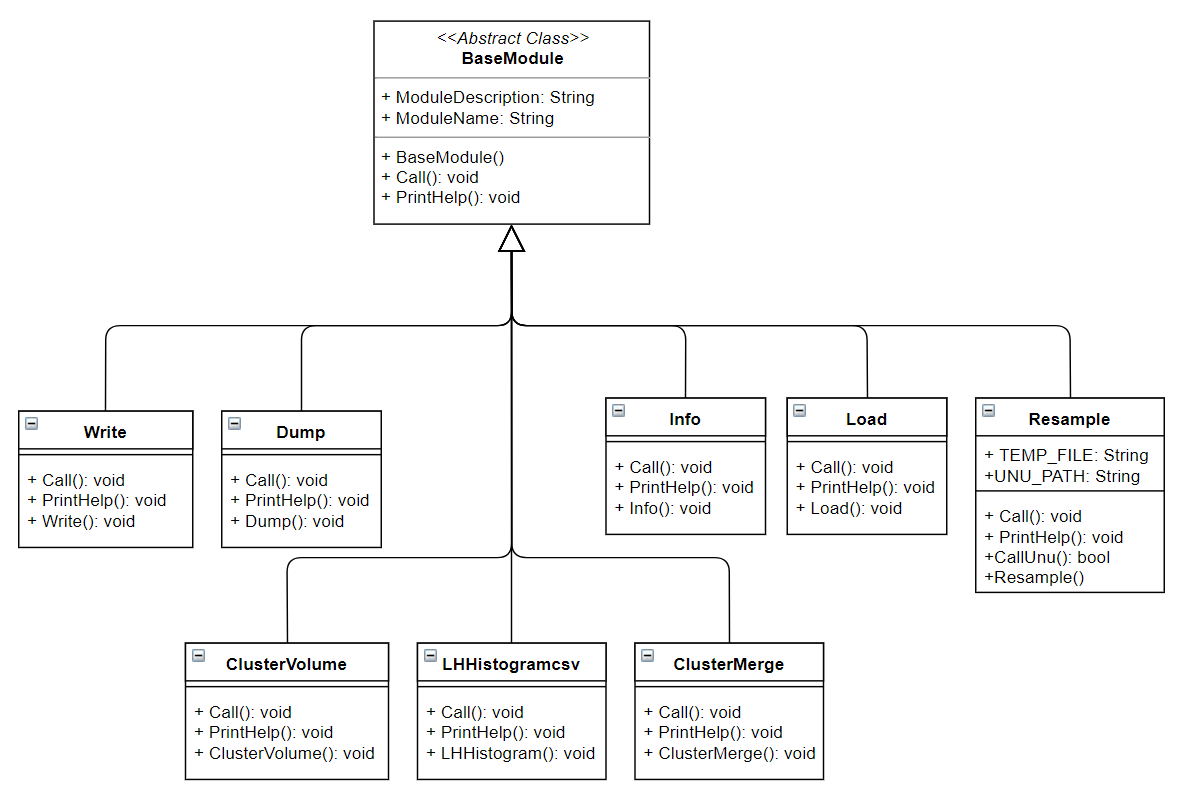
\includegraphics[width=\textwidth]{Logos/Modules_UML.PNG}
\caption{UML-Diagramm über die Module} 
\label{fig:modul_uml} 
\end{figure}


Die Funktionen der Module entsprechen deren Namen und sind im folgenden aufgelistet.


\underline{\textit{Load}}
\newline
Lädt eine .nrrd oder eine binäre Datei.
\newline
\underline{\textit{Dump}}
\newline
Speichert das aktuell geladene Volumen als binäre Datei.
\newline
\underline{\textit{Write}}
\newline
Speichert das aktuell geladene Volumen als .nrrd Datei.
\newline
\underline{\textit{Info}}
\newline
Gibt Informationen über das aktuell geladene Volumen, wie beispielsweise Größe, Minimum, Maximum,.. etc.
\newline
\underline{\textit{Resample}}
\newline
Verändert die Größe des aktuell geladenen Volumens.


Wird der \textit{Dump} Befehl mit einem $u$ am Ende aufgerufen, so wird das Volumen vor dem Speichern zum Typ $unsigned$ $int$ gecastet. Dies geschieht indem auf alle Werte der Betrag des minimalen Wertes aufaddiert wird. Dadurch verschieben sich die Werte so, dass das Minimum bei null liegt, also nur noch positive Zahlen im Volumen vorhanden sind. Dies ist für die Darstellung im Renderer wichtig, da dieser nur mit positiven Zahlen funktioniert. Des Weiteren müssen alle binären Dateien mit dem Suffix .bin.txt gespeichert werden, da Unity die Dateien sonst nicht einlesen kann.


Im Folgenden werden hauptsächlich die Module \textit{LHHistogram}, \textit{ClusterVolume} und \textit{MergeCluster} erläutert, da diese im Laufe dieser Arbeit entstanden sind.


\underline{\textit{LHHistogram}}
\newline
 Berechnet das LH-Histogramm des geladenen Volumens und speichert dieses in einer .csv Datei ab.
\newline
\underline{\textit{ClusterVolume}}
\newline
Kalkuliert die LH-Werte des Volumens und führt hinterher die beiden Clusteringsschritte des Verfahrens aus. Als Ausgabe wird eine binäre Datei eines Volumens gespeichert, in welchem die verschiedenen IDs der Cluster gespeichert sind.
\newline
\underline{\textit{MergeCluster}}
\newline
Verschmilzt die gewünschten IDs mit dem ursprünglichen Volumen.

Das Konzept hinter den IDs wird im laufe dieses Kapitels erklärt. Des Weitern ist das Ergebnis des \textit{MergeCluster} Moduls, ist eine finale binäre Datei, die im Renderer geladen und das Ventrikelsystem visualisiert werden kann. Ein Überblick über den gesamten Aufbau und Ablauf der Implementierung ist in  \autoref{fig:ueberblick} zu sehen.


\begin{figure}
\centering 
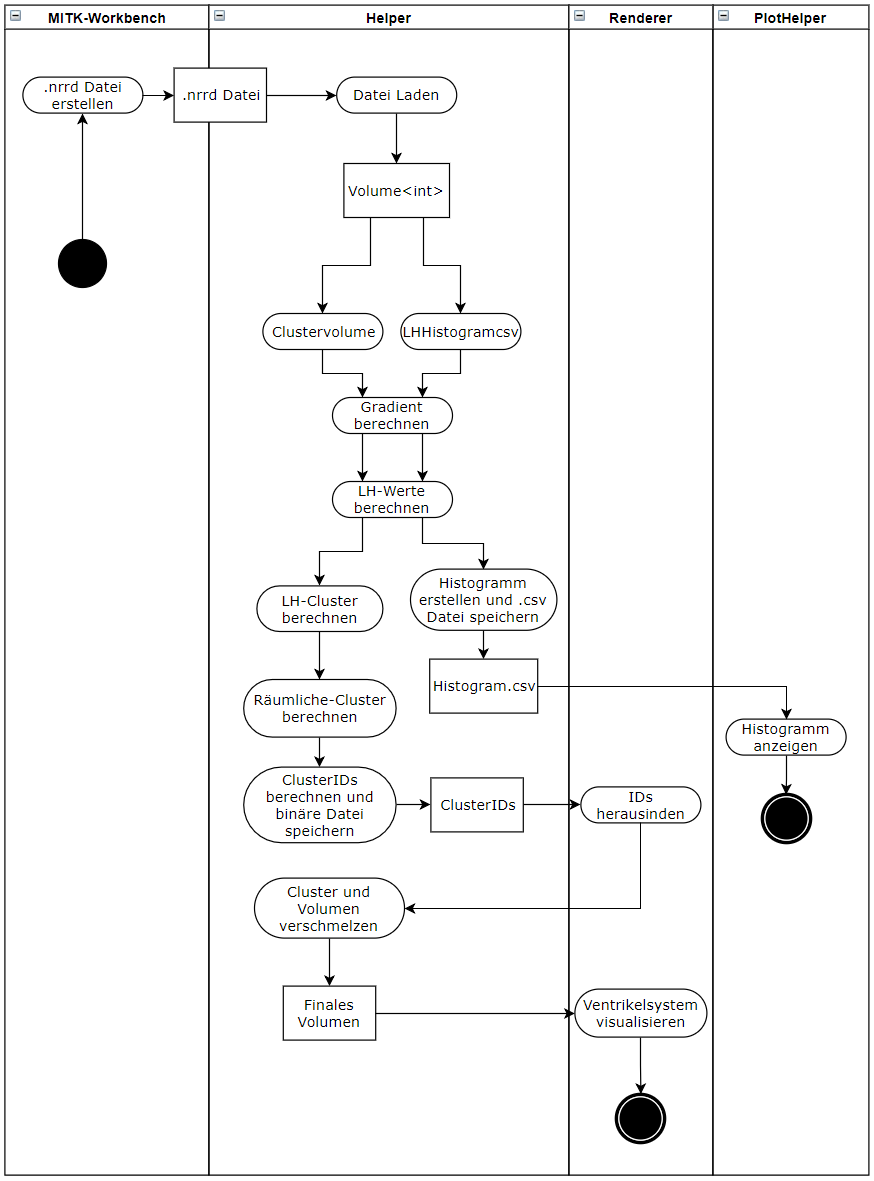
\includegraphics[width=\textwidth]{Logos/Ueberblick2.png}
\caption{Aktivitätsdiagramm über den Prozessablauf} 
\label{fig:ueberblick} 
\end{figure}


Als erstes muss mithilfe des \textit{Load} Moduls ein Volumen geladen werden. Wird anschließend der  \textit{LHHistogram} oder \textit{ClusterVolume} Befehl ausgeführt, beginnt der Ablauf der Berechnung in der statischen \textit{Gradient} Klasse.
Diese ist eine Implementierung des Verfahren von Hong \cite{hong2003method}. Zur Berechnung wird der Funktion \textit{CalcGradientVolume} das Volumen der Intensitätswerte, als \textit{Volume<int>}, als Parameter übergeben. Wie im vorherigen Kapitel besprochen, können die Gradienten nicht für einen Voxel direkt berechnet werden, sondern nur für die Punkte zwischen den Voxeln. Aus diesem Grund ist das Ergebnisvolumen um ein Voxel in jeder Achse kleiner als das Volumen der Intensitätswerte.
\newline
In \autoref{fig:shift} ist dazu ein zweidimensionales Beispiel zu sehen. Die Daten werden hierbei jeweils in der Ecken der Gitter gespeichert. Die Gradienten werden, da es sich um einen zweidimensionalen Fall hält, jeweils in der Mitte von vier benachbarten Punkten berechnet.
Die Dimension der Intensitätswerte ist 5x5, in der Abbildung in schwarz zu sehen. Nachdem die Gradienten berechnet wurden, ist zu erkennen, dass die das Gitter der Gradienten eine Dimension von 4x4 besitzt, in der Abbildung in rot zu sehen.
Als Ergebnis der \textit{CalcGradientVolume} Funktion wird ein Volumen vom Typen \textit{FVector3} zurückgegeben.


\begin{figure}
\centering 
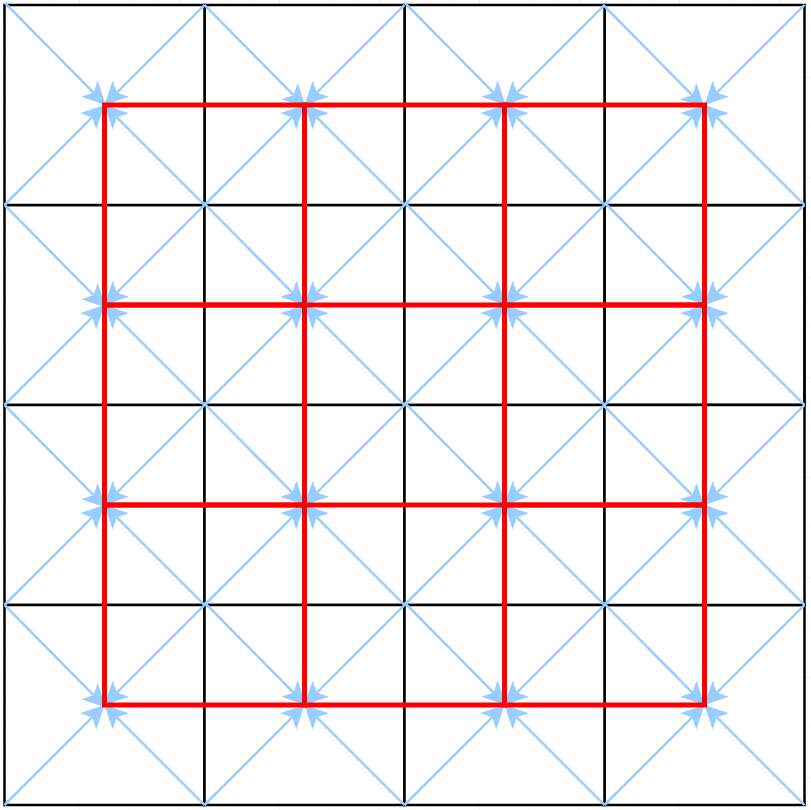
\includegraphics[width=0.75\textwidth]{Logos/VoxelShift.png}
\caption{2D Beispiel warum das Volumen kleiner wird} 
\label{fig:shift} 
\end{figure}


Die Berechnung der LH-Werte findet in der statischen Klasse \textit{LHValues} in der Funktion \textit{LHValueVolume} statt. Als Parameter wird das \textit{FVector3} Volumen der Gradienten aus dem Schritt davor entgegengenommen.
Da für die Berechnung der LH-Werte die Intensitätswerte und die Gradienten am gleichen Punkt vorhanden seien müssen, müssen die Intensitätswerte für das verschobene Volumen der Gradienten berechnet werden. Dazu wurde eine einfache Interpolation durchgeführt, indem von allen 8 Nachbarn eines Punktes die Intensitätswerte aufaddiert und hinterher durch acht geteilt wurden. Hierbei muss jedoch beachtet werden, dass die durch diese Interpolation Informationen verloren gehen.
\newline
Als Ergebnis der Funktion wird ein Volumen von zweier Tupeln zurückgegeben, in denen die Low- und High-Werte gespeichert sind.


Hat der Benutzer das Modul \textit{LHHistogram} aufgerufen, wird im Anschluss das LH-Histogramm in der Klasse \textit{LHHistogramCSV} erstellt und wird von ihr als .csv Datei in einem vom Anwender angegebenen Pfad abgespeichert.
An dieser Stelle kommt das Pythonskript \textit{PlotHelper} zum Einsatz. Dieses lädt die .csv Datei und visualisiert das LH-Histogramm mithilfe einer kalt-zu-heiß-Farbrampe in einem zweidimensionalem Koordinatensystem.
Ein Beispiel davon ist in \autoref{fig:lh_histo} im Kapitel \nameref{sec:implementation} zu sehen. Hierbei ist zu beachten, dass das Histogramm abhängig von der Häufigkeit des Vorkommens eines LH-Wertpaares im Volumen gebildet wird. Diese werden im jeweils dazu passenden Kästchen des Koordinatensystems gespeichert. Dies ist ein simplerer Vorgehen, als das im Paper von Nguyen \cite{nguyen2012clustering} benutzten Erstellen des Histogramms abhängig von einer für jeden Voxel berechneten Gewichtung.
\newline
Da die Arbeit an der Implementierung zeitlich beschränkt war, wurde diese Gewichtung, die einzig und allein einer genaueren Darstellung des für das Verfahren irrelevante LH-Histogramm dient, vernachlässigt. Die Gewichtung ist für das Clustering belanglos, da dort ein Histogramm wie eben beschrieben, abhängig von der Häufigkeit der LH-Werte verwendet wird.
Bei der Erstellung des Histogramms im \textit{LHHistogram} Modul wird weiterhin der Logarithmus der Anzahl der Einträge jedes Kästchens genommen. Dies geschieht aus dem Grund der großen Diskrepanz zwischen der Anzahl der Einträge an den meisten Stellen im Histogramm im Vergleich zu dem Maximum. Dies lässt bei der Darstellung mit einer Farbrampe fast alles mit der Farbe des Minimums anzeigen. Da die Logarithmusfunktion für schnell wachsende Zahlen nur sehr langsam steigt, eignet sie sich dafür, diesen großen Unterschied anzupassen.


Wurde das \textit{ClusterVolume} Modul aufgerufen, wird mit den beiden Clusteringschritten fortgefahren. Die Berechnung der LH-Cluster findet in der \textit{LHClustering} Klasse statt. Hierbei nimmt die Funktion \textit{ComputeLHClusters} das Volumen mit den LH-Werten entgegen und rechnet dieses aus Performancegründen, mit dem gleichen Vorgehen, welches im \textit{LHHistogram} Modul benutzt wurde, in ein Histogramm um. Jedoch wird nicht der Logarithmus der Einträge genommen. Dieser Schritt könnte gespart werden, wenn die Methode \textit{LHValueVolume} direkt ein Histogramm als Rückgabewert liefern würde. Eine solche Änderung würde auch das \textit{LHHistogram} Modul verbessern, da damit die Umrechnung, die in dieser Klasse geschieht, ebenso gespart werden könnte.
\newline
Als Ergebnis der Clusteringfunktion wird eine Liste der Cluster zurückgegeben. Ein Cluster besteht hierbei aus einer Liste von \textit{IVector3}. Die Cluster werden nur als Liste der räumliche Informationen der Voxel gespeichert, da für den nächsten Clusteringschritt  lediglich diese Information benötigt wird. 


Anschließend geht es in der Funktion \textit{ComputeIDs} der \textit{SpatialClustering} Klasse mit der Berechnung der räumlichen Cluster weiter. Diese werden mit einer ähnlichen Implementierung wie in der \textit{LHClustering} Klasse kalkuliert. Diesmal wird jedoch kein Histogramm für das Clustering erstellt, sondern die Berechnung direkt auf den übergebenen Listen durchgeführt. Des Weiteren wurde eine Mindestgröße für die entstehenden Cluster festgelegt, um kleine unbedeutende Cluster zu entfernen. Als Ergebnis wird erneut eine Liste von Listen vom Typ \textit{IVector3} zurückgegeben.


Nachdem alle Cluster kalkuliert wurden, werden sie in der \textit{ClusterVolume} Klasse in einem Volumen gespeichert. Jeder Cluster bekommt dabei zunächst eine einzigartige ID. Die IDs beginnen bei eins und werden hochgezählt. Anschließend wird das Volumen mit den verschiedenen IDs gefüllt. Dies geschieht indem für jeden Cluster an den Positionen der Punkte die jeweilige ID gespeichert wird. Alle anderen Voxeln des Clustervolumens wird der Wert null zugewiesen.
Dieses Volumen wird als binäre Datei gespeichert und ist das Ergebnis des \textit{ClusterVolume} Moduls. Es ist bei diesem Modul sehr wichtig, dass es, wie es bei dem \textit{Dump} Befehl möglich ist, mit einem $u$ am Ende aufgerufen wird, da das Ergebnis sonst nicht vom Renderer eingelesen werden kann.


Das Ergebnis muss anschließend vom Nutzer in Unity geladen werden. Hierbei kommt die in dieser Arbeit vorgenommenen Anpassung am Renderer zum Einsatz.
Hier hat der Benutzer durch die Erweiterung die Möglichkeit einen speziellen Wert oder einen Wertebereich hervorzuheben. Da das Volumen lediglich die IDs als Werte gespeichert hat und sonst nur aus nullen besteht, werden wenn ein Wert vom User angegeben wird, die Voxel die zum Cluster der jeweiligen ID gehören hervorgehoben.
Mithilfe dessen muss der Anwender alle Cluster die zum Ventrikelsystem gehören finden und sich deren IDs zu notieren.


Hat er dies getan kann er mit dem \textit{MergeCluster} Modul des Helpers das Ergebnis zusammenfügen und die finale Visualisierung erstellen. Beim Aufruf muss das Intensitätsvolumen bereits geladen sein und der Benutzer das Clustervolumen, die ausgewählten IDs und ein Zielpfad als Parameter übergeben. In der \textit{Call} Methode der \textit{MergeCluster} Klasse wird anschließend an den Stellen im Volumen, an denen die entsprechenden IDs gespeichert sind, die Werte im Intensitäsvolumen auf 5000 gesetzt.
Nach dem beschriebenen Verschieben aller Werte ins positive, liegt der maximale Intensitätswert bei ungefähr 4500. Folglich erhöht das Hinzufügen des Wertes 5000 das Maximum des Volumens, und damit die Darstellung im Renderer nur gering, und lässt es zu, die segmentierten Bereiche klar vom Rest abzugrenzen. Dieses Volumen wird erneut als binäre Datei im Zielpfad abgespeichert.


Als letzten Schritt kann der Benutzer die finale binäre Datei in Unity laden. Anschließend muss er den \textit{SpecificValue} Modus auswählen und den hervorzuhebenden Wert auf 5000 setzten.













































